\section*{Domácí úloha 2}

\subsection*{Příklad č.~6}

Najděte všechny podgrupy $(\mathbb{Z}_{6}, \oplus)$. Které z nich jsou normální? Sestrojte příslušné faktorové grupy.

\begin{eqnarray*}
\mathbb{Z}_{6} &=& \lbrace 0, 1, 2, 3, 4, 5 \rbrace \\ 
a \oplus b &=& (a + b) \mod 6
\end{eqnarray*}

\minipage{0.50\textwidth}
\begin{center}
\begin{tabular}{|c|c|c|c|c|c|c|}
\hline 
$\oplus$ & 0 & 1 & 2 & 3 & 4 & 5\\ 
\hline 
0        & 0 & 1 & 2 & 3 & 4 & 5 \\
\hline 
1        & 1 & 2 & 3 & 4 & 5 & 0 \\ 
\hline 
2        & 2 & 3 & 4 & 5 & 0 & 1 \\ 
\hline 
3        & 3 & 4 & 5 & 0 & 1 & 2 \\ 
\hline 
4        & 4 & 5 & 0 & 1 & 2 & 3 \\ 
\hline 
5        & 5 & 0 & 1 & 2 & 3 & 4 \\ 
\hline 
\end{tabular} 
\end{center}
\endminipage
\minipage{0.50\textwidth}
\begin{itemize}
\item Jednotkový prvek je $0$.
\item Inverzní prvek $a \oplus a^{-1} = 0$.
\end{itemize}
$
\left.{\begin{array}{l}
0 \oplus 0 = 0 \\
0 \oplus 1 = 1 \\
0 \oplus 2 = 2 \\
0 \oplus 3 = 3 \\
0 \oplus 4 = 4 \\
0 \oplus 5 = 5 \\
\end{array}}\right\} = \mathbb{Z}_{6}
$
\endminipage

\minipage{0.16\textwidth}
\begin{eqnarray*}
0 \oplus 0 &=& 0
\end{eqnarray*}
\endminipage
\minipage{0.16\textwidth}
\begin{eqnarray*}
0 \oplus 1 &=& 1 \\
1 \oplus 1 &=& 2 \\
2 \oplus 1 &=& 3 \\
3 \oplus 1 &=& 4 \\
4 \oplus 1 &=& 5 \\
5 \oplus 1 &=& 0 
\end{eqnarray*}
\endminipage
\minipage{0.16\textwidth}
\begin{eqnarray*}
0 \oplus 2 &=& 2 \\
2 \oplus 2 &=& 4 \\
4 \oplus 2 &=& 0
\end{eqnarray*}
\endminipage
\minipage{0.16\textwidth}
\begin{eqnarray*}
0 \oplus 3 &=& 3 \\
3 \oplus 3 &=& 0
\end{eqnarray*}
\endminipage
\minipage{0.16\textwidth}
\begin{eqnarray*}
0 \oplus 4 &=& 4 \\
4 \oplus 4 &=& 2 \\
2 \oplus 4 &=& 0
\end{eqnarray*}
\endminipage
\minipage{0.16\textwidth}
\begin{eqnarray*}
0 \oplus 5 &=& 5 \\
1 \oplus 5 &=& 0 \\
2 \oplus 5 &=& 1 \\
3 \oplus 5 &=& 2 \\
4 \oplus 5 &=& 3 \\
5 \oplus 5 &=& 4 
\end{eqnarray*}
\endminipage

\begin{eqnarray*}
T_{1} &=& \lbrace 0 \rbrace \\
T_{2} &=& \mathbb{Z}_{6} = \\ &=& \lbrace 0, 1, 2, 3, 4, 5 \rbrace \\
T_{3} &=& \lbrace 0, 2, 4 \rbrace \\
T_{4} &=& \lbrace 0, 3 \rbrace \\
T_{5} &=& T_{3} \\
T_{6} &=& T_{2}
\end{eqnarray*}

\subsection*{Příklad č.~7}

Najděte všechny distributivní svazy o 5 prvcích.

\subsection*{Příklad č.~8}

V Booleově algebře $(X, \oplus, \odot, {}^{\prime}, 0, 1)$ zjednodušte výrazy:

\begin{eqnarray*}
(a \oplus c) \oplus (c \oplus b) \oplus (b \oplus a) &=&
a \oplus a \oplus b \oplus b \oplus c \oplus c = \\ &=&
a \oplus b \oplus c
\end{eqnarray*}

\begin{eqnarray*}
(x \odot y) \oplus (x \odot z) \oplus (x^{\prime} \odot z^{\prime})^{\prime} &=&
(x \odot y) \oplus (x \odot z) \oplus (x \oplus z) = \\ &=&
[\lbrace x \odot (y \oplus z) \rbrace \oplus x] \oplus z = \\ &=&
[x \oplus x] \oplus z = \\ &=&
x \oplus z
\end{eqnarray*}

\begin{eqnarray*}
(x^{\prime} \oplus y^{\prime})^{\prime} &=&
x \odot y
\end{eqnarray*}

\subsection*{Příklad č.~9}

Buď $G$ úplný graf o $n$ vrcholech. Určete počet cest délky 2, které začínají v pevně zvoleném vrcholu $a$ a končí v jiném pevně zvoleném vrcholu $b$. Kolik existuje takových cest délky 3? Zobecněte tento výsledek pro libovolné $k$, kde $1 \leq\ k < n$.

\subsection*{Příklad č.~10}

Nakreslete graf se šesti vrcholy, který lze nakreslit jedním uzavřeným tahem, ale v němž neexistuje hamiltonovská kružnice. Náležitě zdůvodněte, že tento graf má požadované vlastnosti. \\

\begin{center}
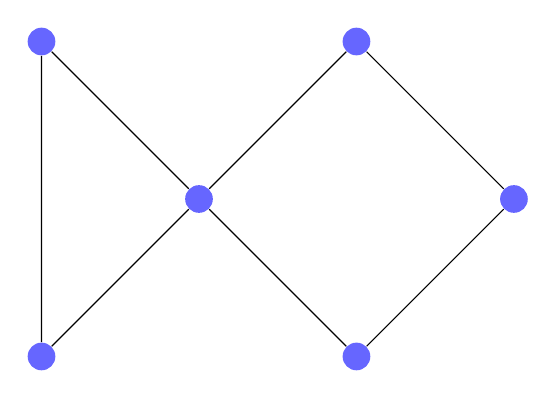
\begin{tikzpicture}[main_node/.style={circle,fill=blue!60,minimum size=1em,inner sep=3pt]}]
    \node[main_node] (1) at (-2, -2) {};
    \node[main_node] (2) at (-2, 2) {};
    \node[main_node] (3) at (0, 0) {};
    \node[main_node] (4) at (2, 2) {};
    \node[main_node] (5) at (4, 0) {};
    \node[main_node] (6) at (2, -2) {};
    \draw (1) -- (2) -- (3) -- (4) -- (5) -- (6) -- (3) -- (1);
\end{tikzpicture} \\
\end{center}
